\documentclass[review]{elsarticle}

\usepackage{lineno,hyperref}

\usepackage{graphicx}% Include figure files
\usepackage{dcolumn}% Align table columns on decimal point
\usepackage{amsmath}
\usepackage{amssymb}
\usepackage{epstopdf}
\usepackage{multirow}
\usepackage{color}
%\usepackage{hepparticles} % particle names
%\usepackage{hepnames} % shortcuts for lots of particle names
\usepackage[alsoload=hep]{siunitx}
\sisetup{ per-mode=symbol}


\graphicspath{{figures/}}
\modulolinenumbers[5]

\journal{}
\bibliographystyle{elsarticle-num}

\begin{document}


%%%%%%%%%%%%%%%%%%%%%%%%%%%%%%%%%%%%%%%%%%%%%%%%%%%%%%%%%%%%%%%%%%%%%%%%%%%%%%%%%%%%%%%%%%%%%%%%%%%
\begin{frontmatter}

\title{A backward angle detector for high momentum neutrons}

%% Group authors per affiliation:
\author{Authors\corref{mycorrespondingauthor}}
\address{Addresses}

%%%%%%%%%%%%%%%%%%%%%%%%%%%%%%%%%%%%%%%%%%%%%%%%%%%%%%%%%%%%%%%%%%%%%%%%%%%%%%%%%%%%%%%%%%%%%%%%%%%
\author[]{}
\ead[]{}

\begin{abstract}
We present a bunch of stuff about BAND and how awesome it is.
\end{abstract}

\begin{keyword}
\end{keyword}
\end{frontmatter}

%%%%%%%%%%%%%%%%%%%%%%%%%%%%%%%%%%%%%%%%%%%%%%%%%%%%%%%%%%%%%%%%%%%%%%%%%%%%%%%%%%%%%%%%%%%%%%%%%%%
\linenumbers

\section{Introduction}
\begin{itemize}
\item Quick physics background about tagged DIS measurements and EMC/SRC
\item Quick overview of CLAS12
\item broad/generic of BAND
\end{itemize}


The CLAS12 (Cebaf Large Angle Spectrometer)[ADD REF] in Jefferson Lab's HallB experimental hall is a multi-purpose spectrometer to detect charged and neutral particles. It covers angles from xx to xx and momenta from xx to xx for the different particles. For our physics of interest, it is necessary to detect recoil neutrons with momenta above \SI{200/250}{\mega\eVperc} at backward angles. Therefore, a new detector has been build to detect these neutrons, the Backward Angle Neutron Detector (BAND). 

Mention here general design considerations of BAND -- efficiency for XX momenta and coverage of XX angles with resolutions XX and design space XX.

%%%%%%%%%%%%%%%%%%%%%%%%%%%%%%%%%%%%%%%%%%%%%%%%%%%%%%%%%%%%%%%%%%%%%%%%%%%%%%%%%%%%%%%%%%%%%%%%%%%

\section{Design of the BAND}

\begin{itemize}
\item geometry
\begin{figure}[thb]
\centering
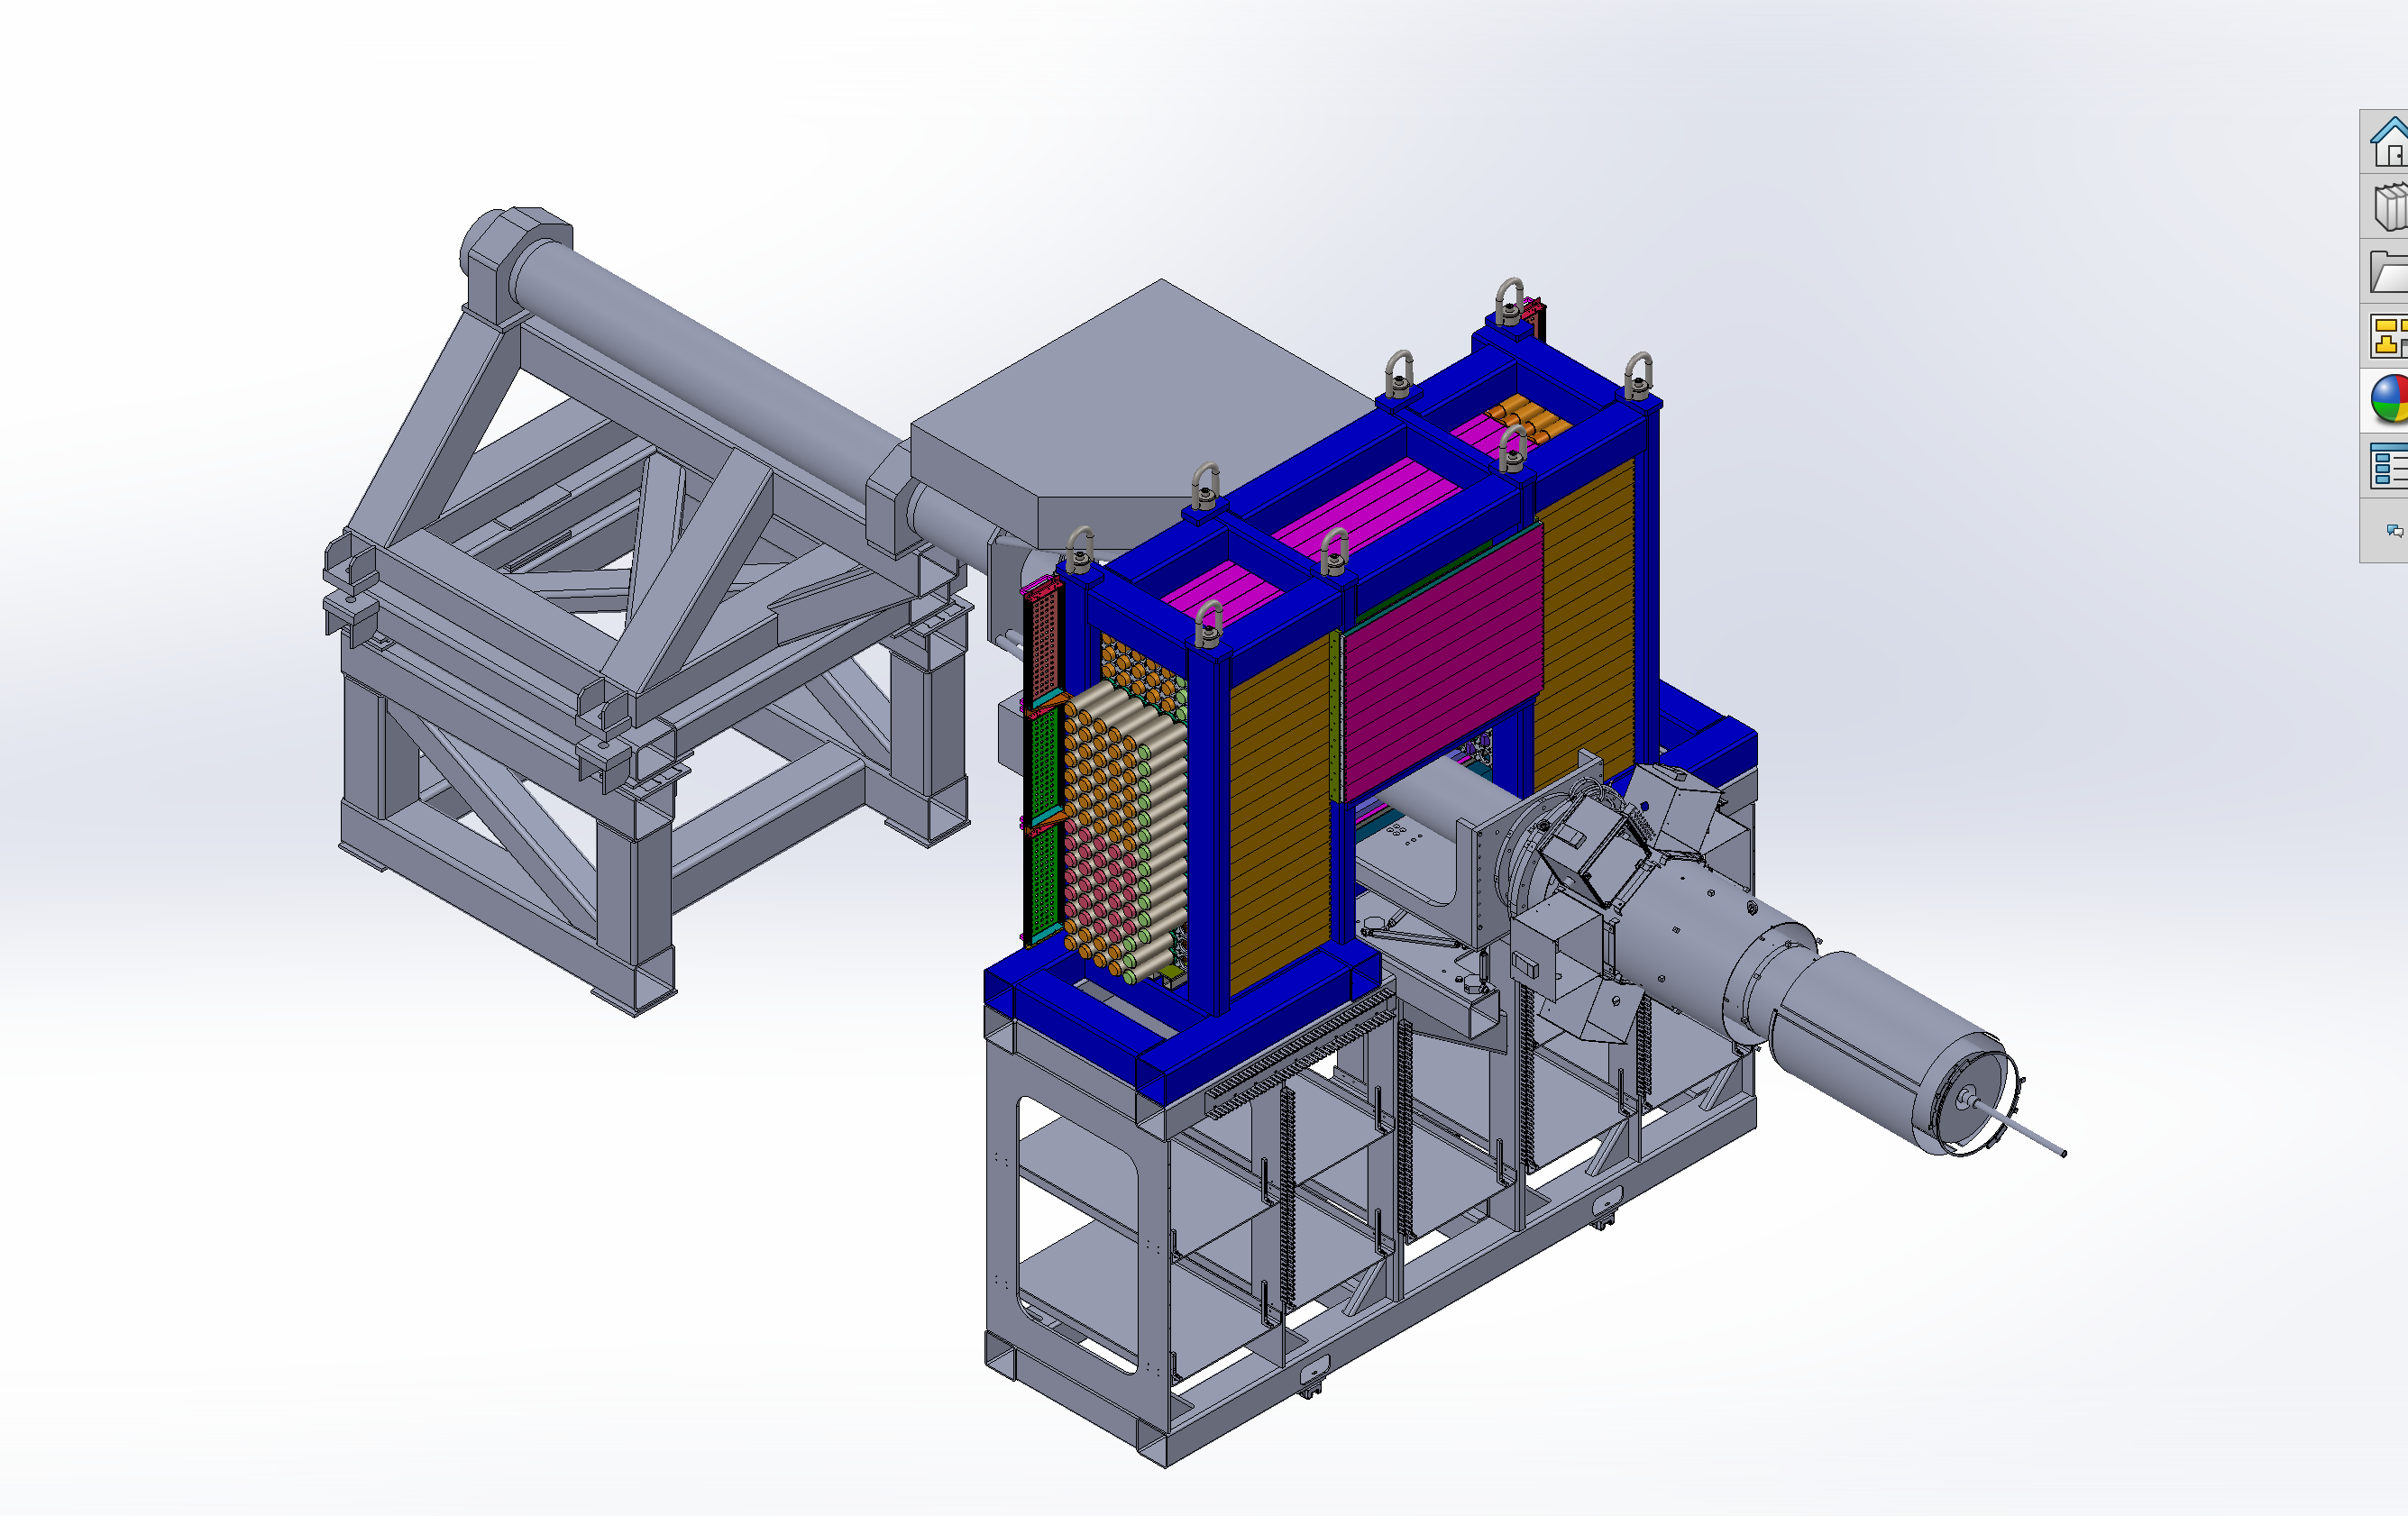
\includegraphics[width=0.48\textwidth]{BandInContext1.png}
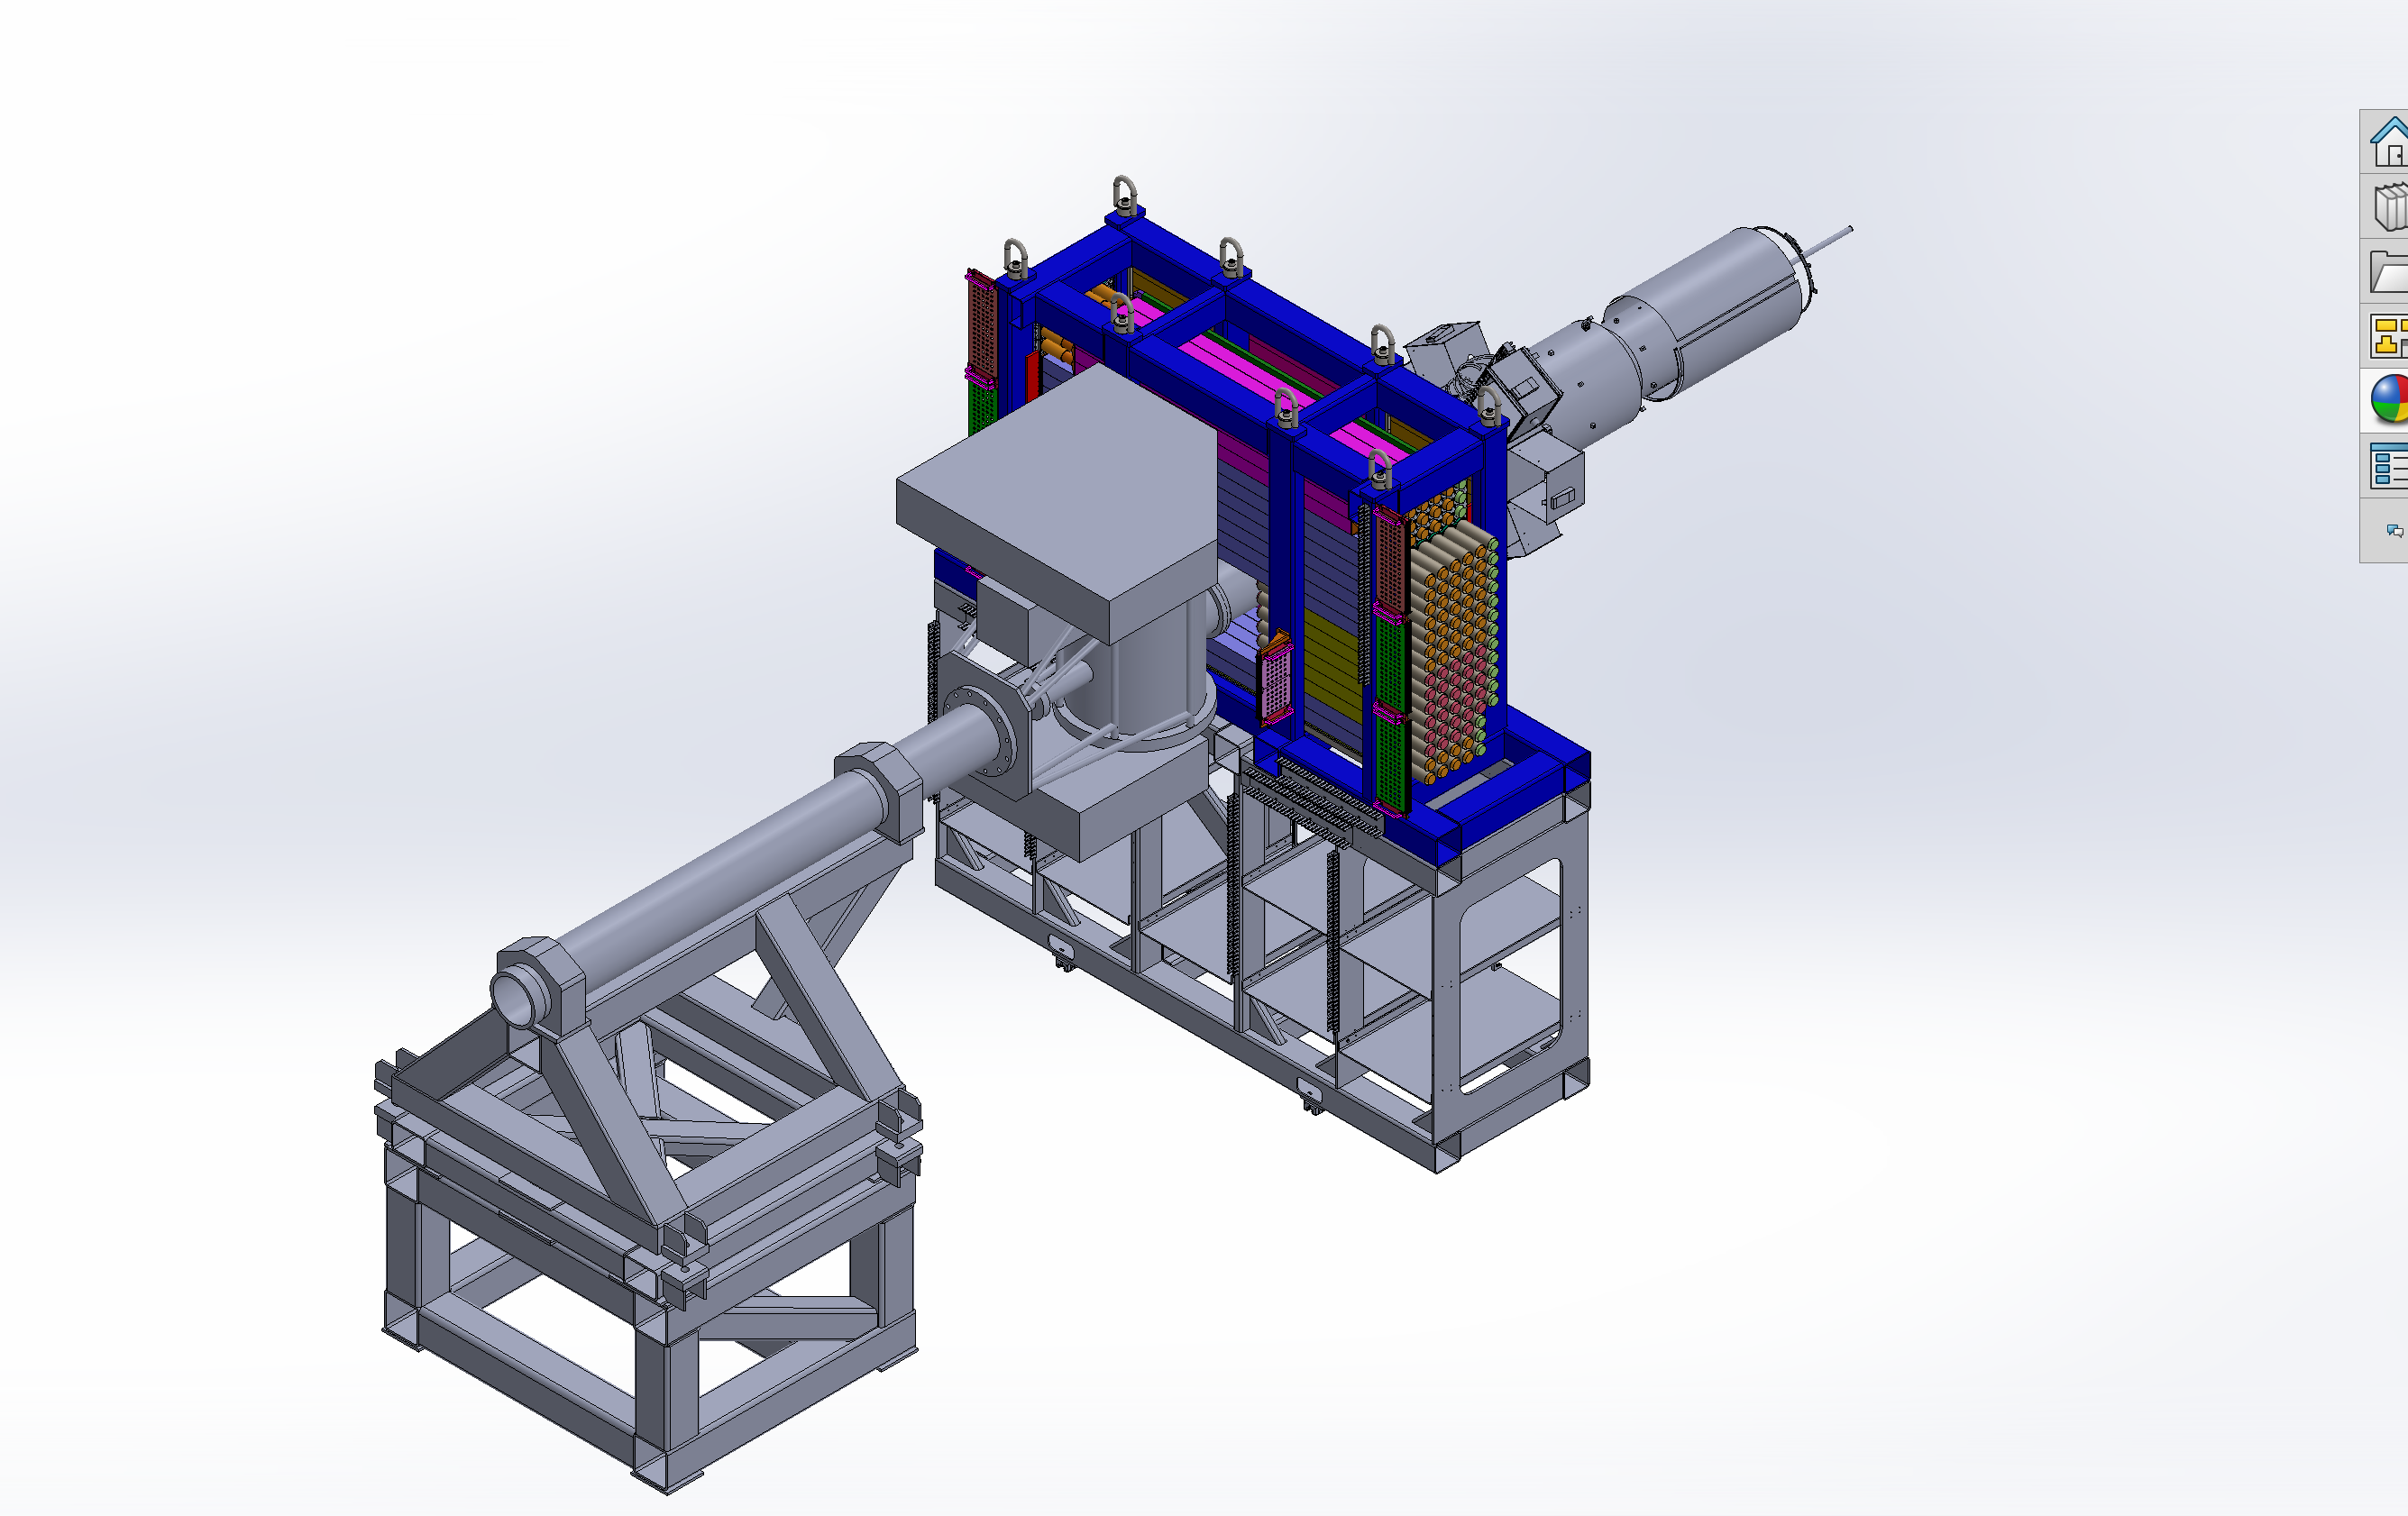
\includegraphics[width=0.48\textwidth]{BandInContext2.png}
 \caption{TODO: better picture, I don't like the options on the CAD drawing. The BAND detector is shown with its surroundings: CLAS12 target, beam line and Silicon Vertex Tracker cart. (Left) Beam is coming from top left. (Right) Beam is coming from bottom left. }
  \label{fig:bandcontext}
\end{figure}
The BAND detector consist of plastic scintillators made from  EJ-200 scintillant. Each bar in the active detector area has a cross section of $7.2 \times 7.2\,\mathrm{cm}^{2}$. In total there are 116 scintillator bars, arranged in 5 layers with 18 vertically stacked bar. The arrangement of the bars is shown in Fig. \ref{fig:barlayout}. The bottom rows are only arranged in four layers due to obstruction from surrounding frames.

\begin{figure}[htb]
\centering
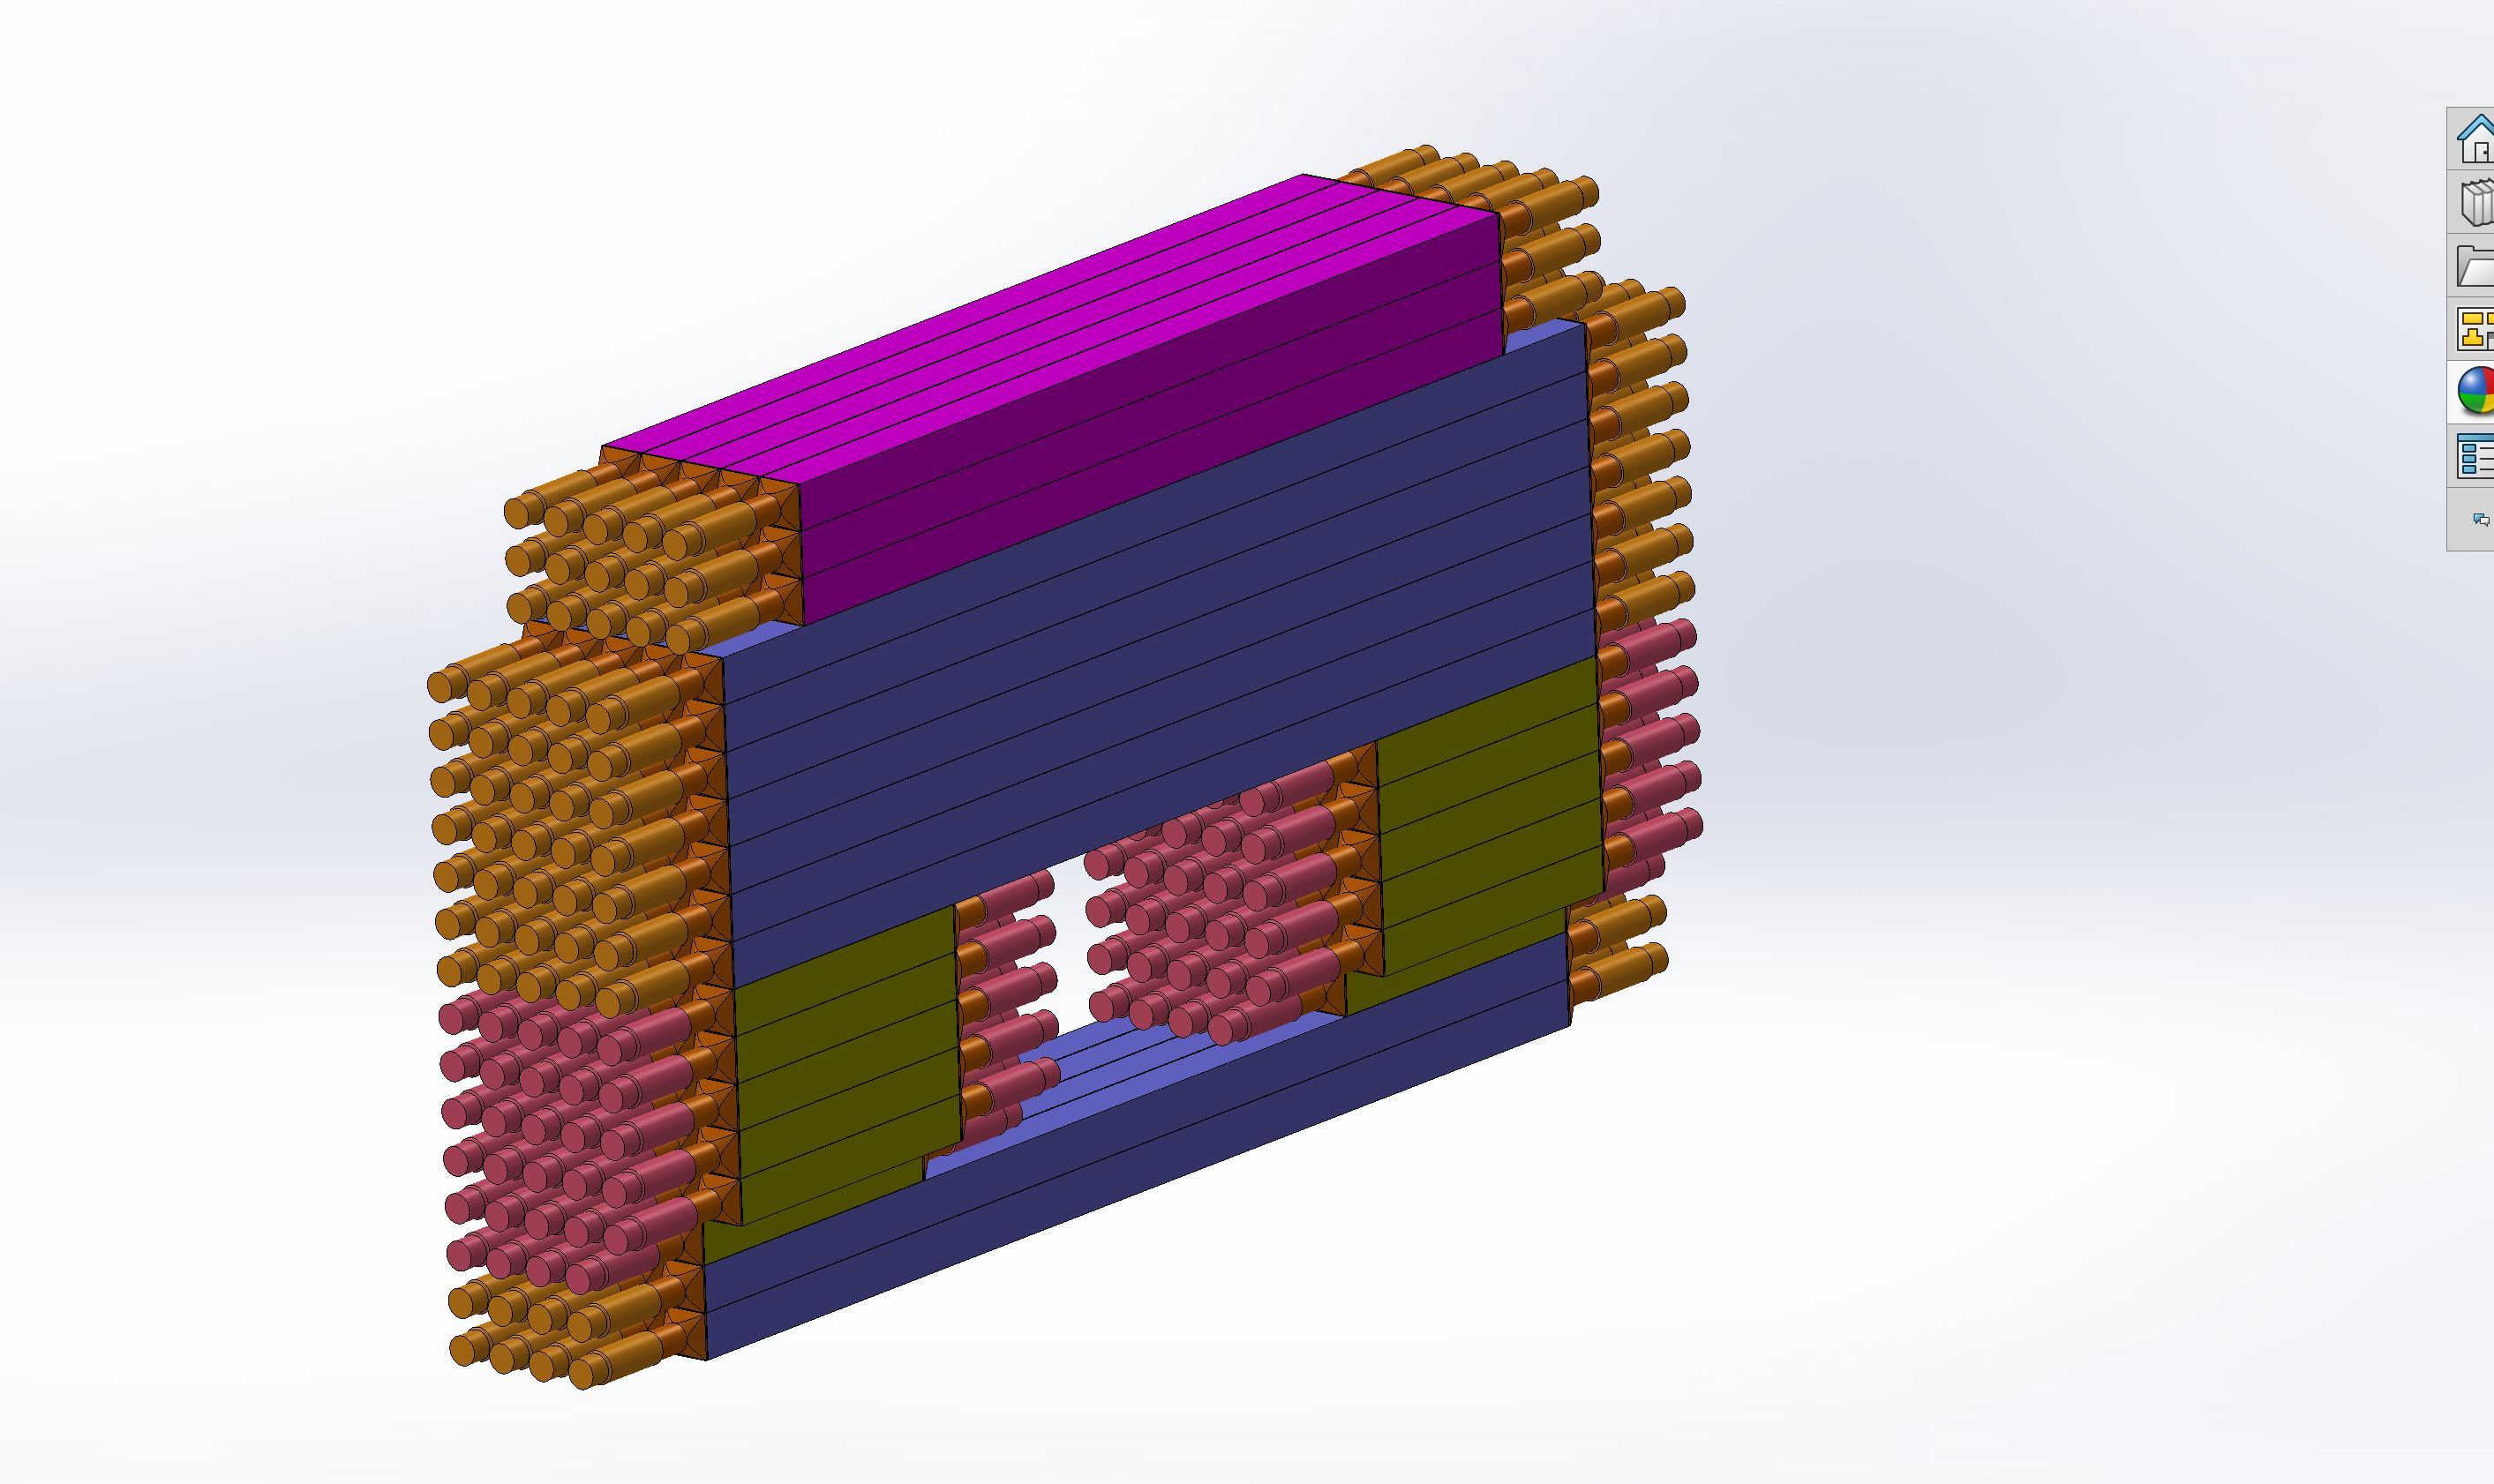
\includegraphics[width=0.48\textwidth]{Band01.png}
  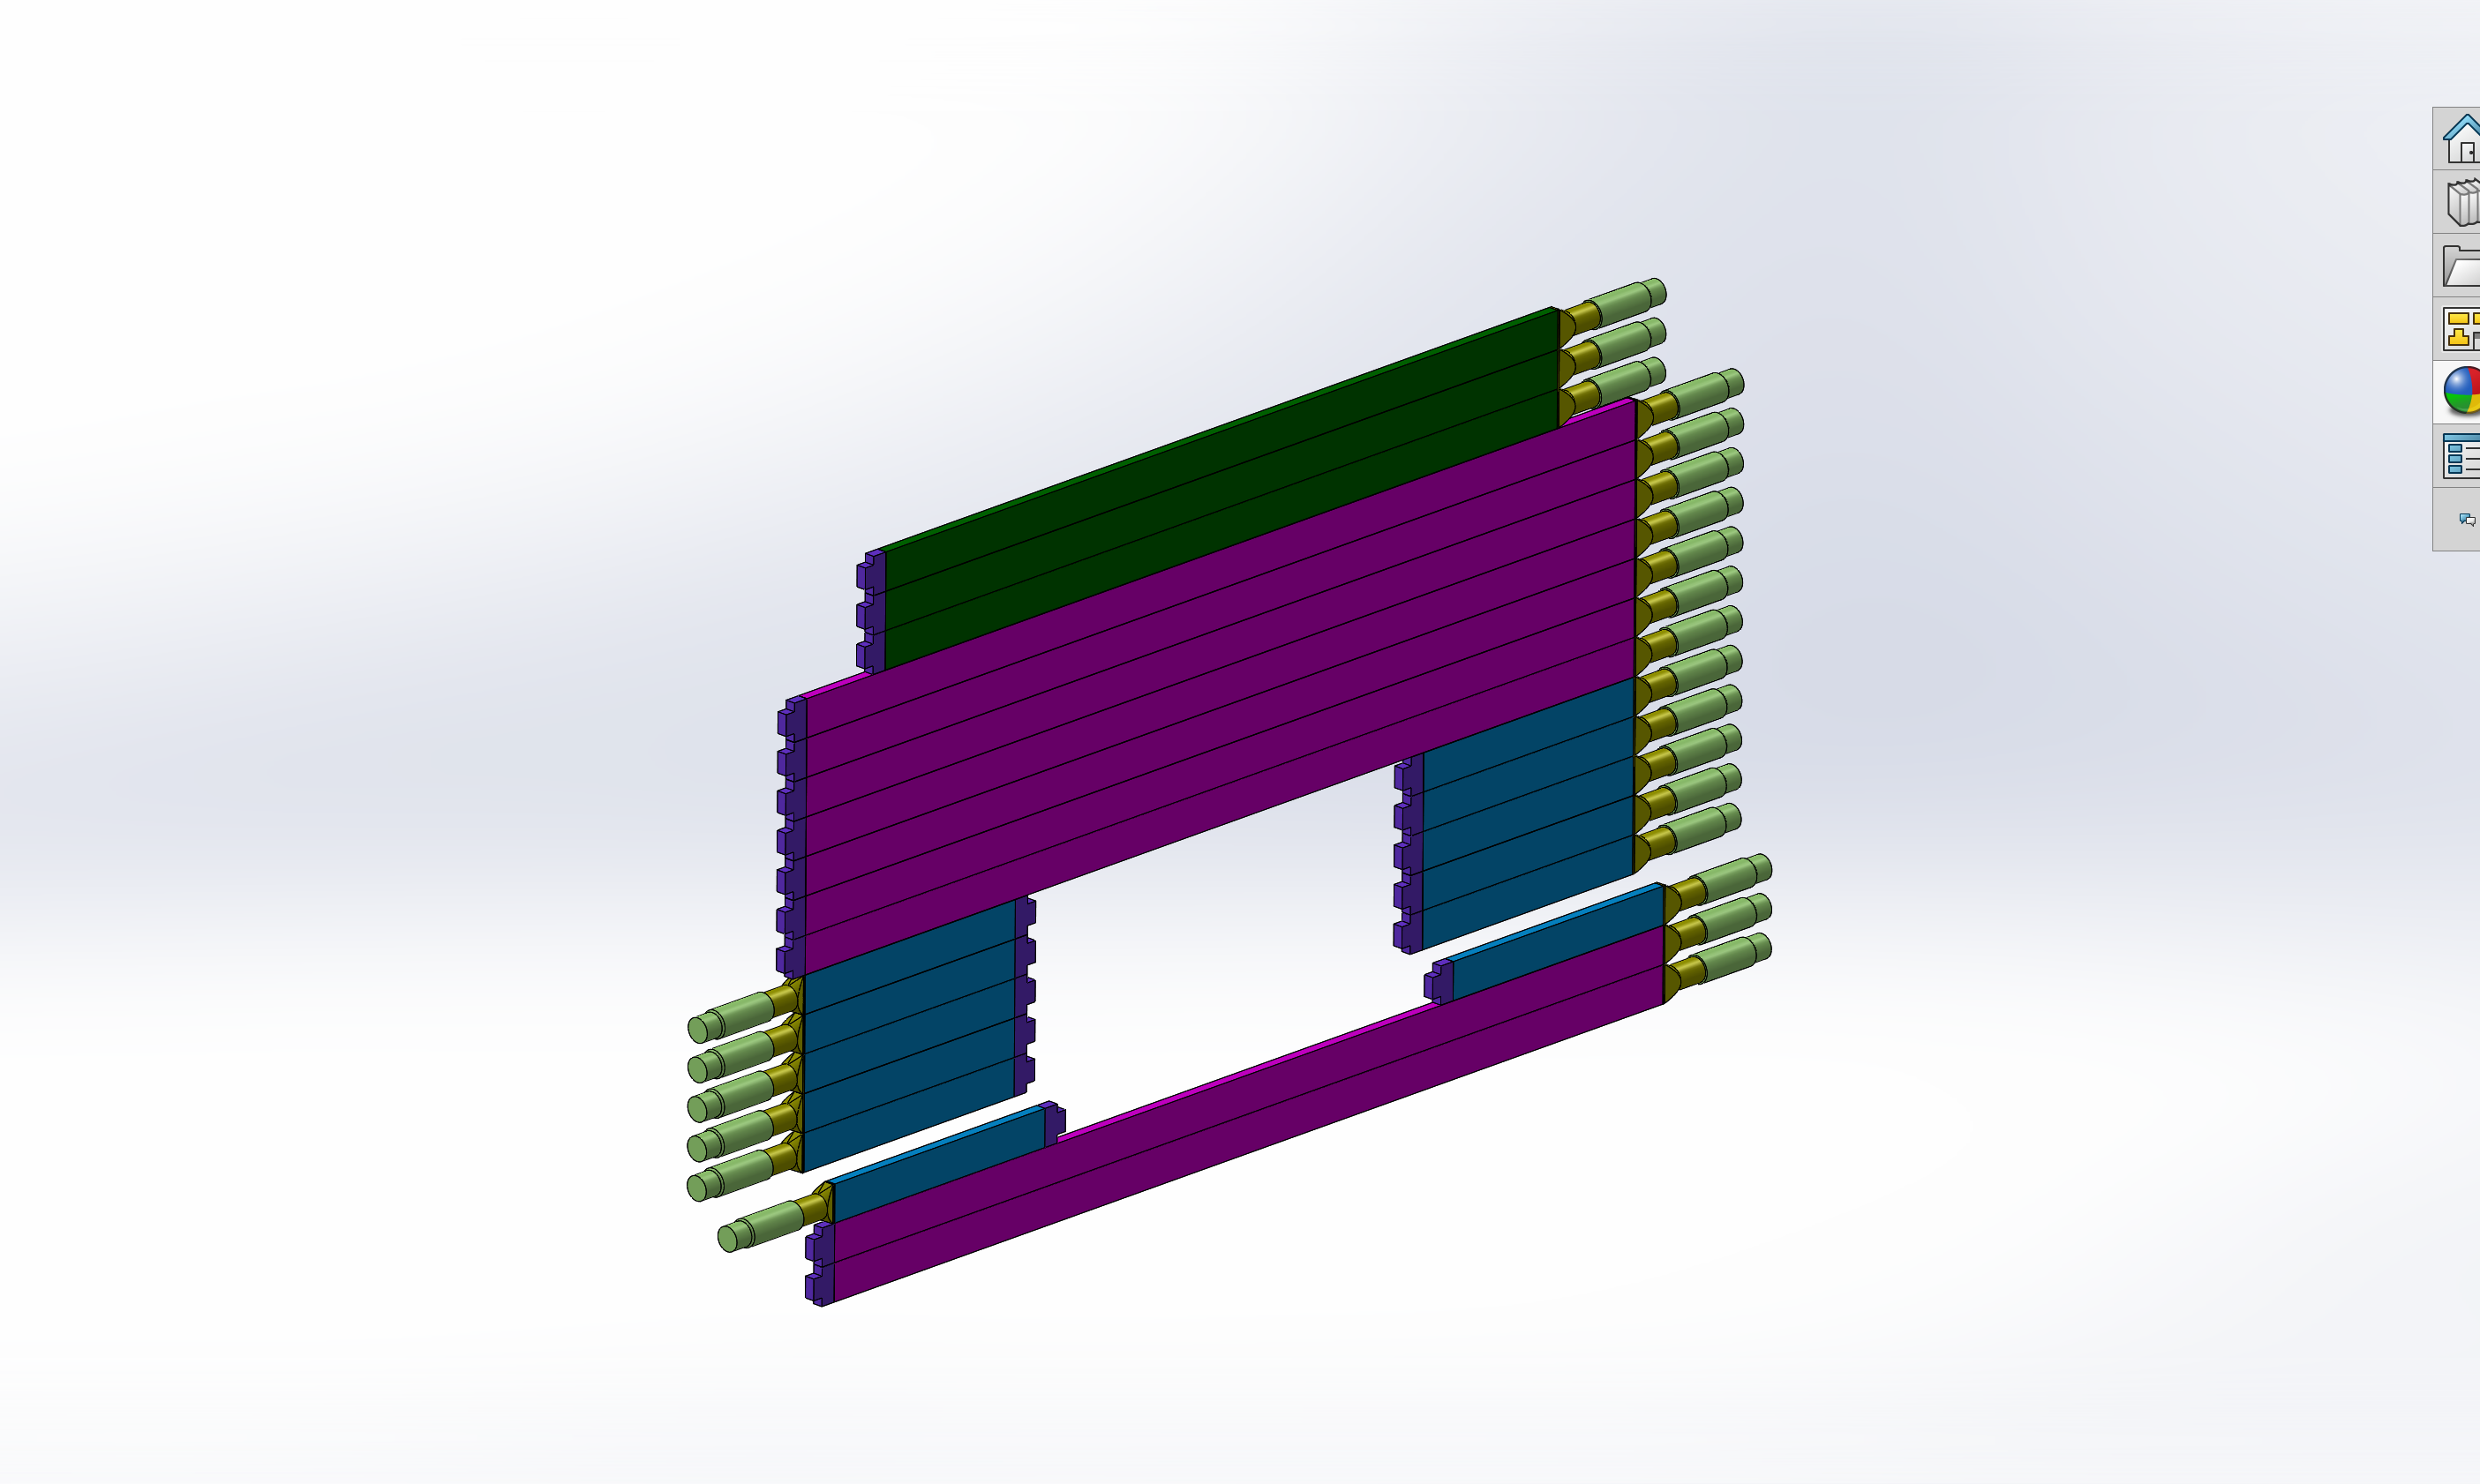
\includegraphics[width=0.48\textwidth]{BandVeto.png}
 \caption {(Left) Isometric view of the active BAND detector volume. The geometry is comprised of 5 layers of 18 vertically stacked bars. The magenta bars (top) are $164\,\mathrm{cm}$ long, the blue bars are $202\,\mathrm{cm}$ long while the shorter green bars around the beam hole are $51\,\mathrm{cm}$ long. Every bar is read out on both sides by a PMT. (Right) Isometric view of the BAND veto layer. It is similar to the active area of BAND. The bars have the same length as the bars shown in Fig. \ref{fig:barlayout}. Every bar is read out on one side by a PMT.}
  \label{fig:vetolayout}
\end{figure}
Three different long bars are used in the detector: 15 bars with a length of $164\,\mathrm{cm}$ (magenta in Fig. \ref{fig:barlayout}), 43 bars with a length of $202\,\mathrm{cm}$ (blue in Fig. \ref{fig:barlayout}) and 58 short bars with a length of $51\,\mathrm{cm}$ (green in Fig. \ref{fig:barlayout}). The short bars are necessary for the hole for the beam line and target installation. The total thickness is $36\,\mathrm{cm}$ gives a neutron detection efficiency of about 30\%.

All bars are read-out on both sides by PMTs (100 Hamamatsu R7724  [ADD REF] and 132 ET 9214  [ADD REF]) giving a total of 232 active channels. Since the PMTs are placed in the fringe field region of the solenoid, and they are encased in a cylindrical shielding made up by a \SI{2}{\milli\metre} thick layer of mu-metal.

In front of the first active layer of BAND, a veto layer is installed with 24 scintillators bars which are read-out only on one side by Thorne EMI 9954KB PMTs [ADD REF]. The bars have a cross section of $2 \times 7.2\,\mathrm{cm}^{2}$. The bars in the veto layer have the same length as the bars of one layer of the active detector area. The veto layer is shown in Fig. \ref{fig:vetolayout}.


\item Scint material
\item which PMTs / why
\begin{figure}[h!]
\centering
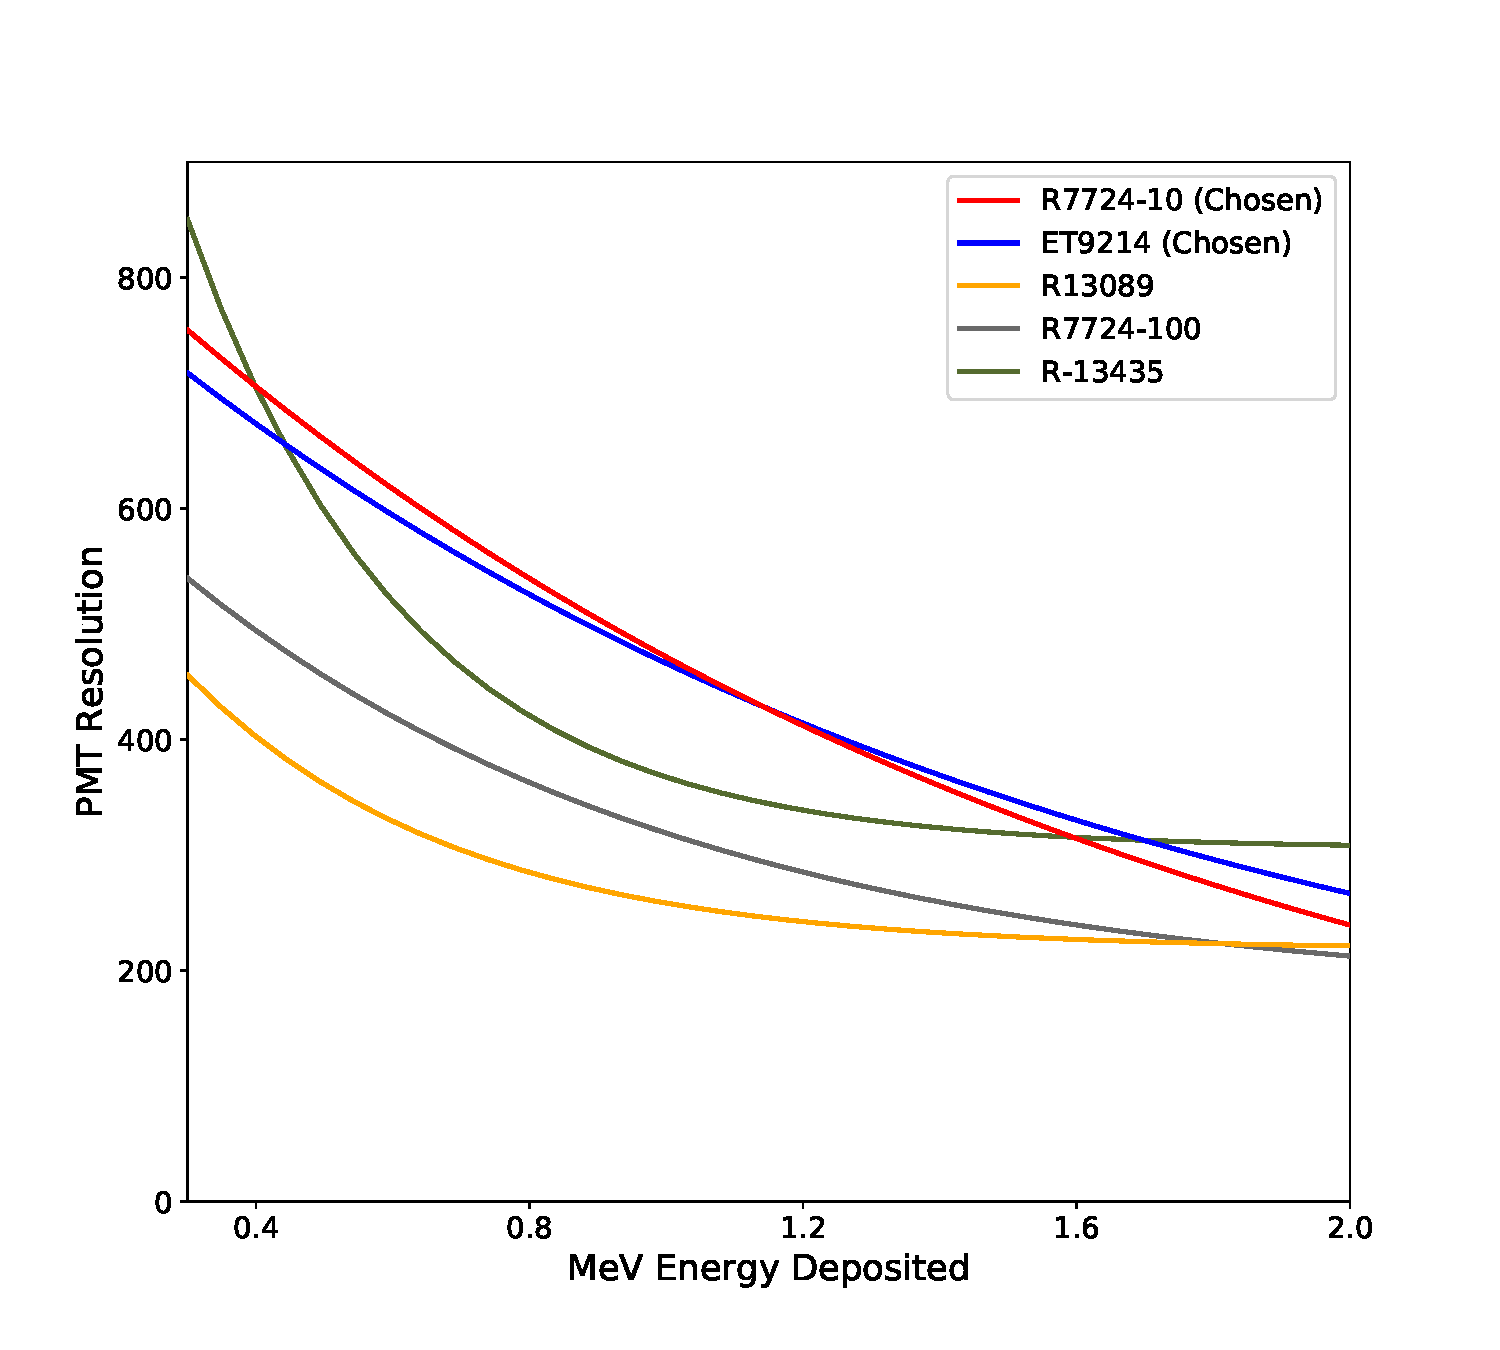
\includegraphics[width=0.7\textwidth]{test-stand/test-resolutions.pdf}
\caption{}
\label{fig:bandpmts}
\end{figure}

\item mu metal study
\item light guides
\begin{figure}[h!]
\centering
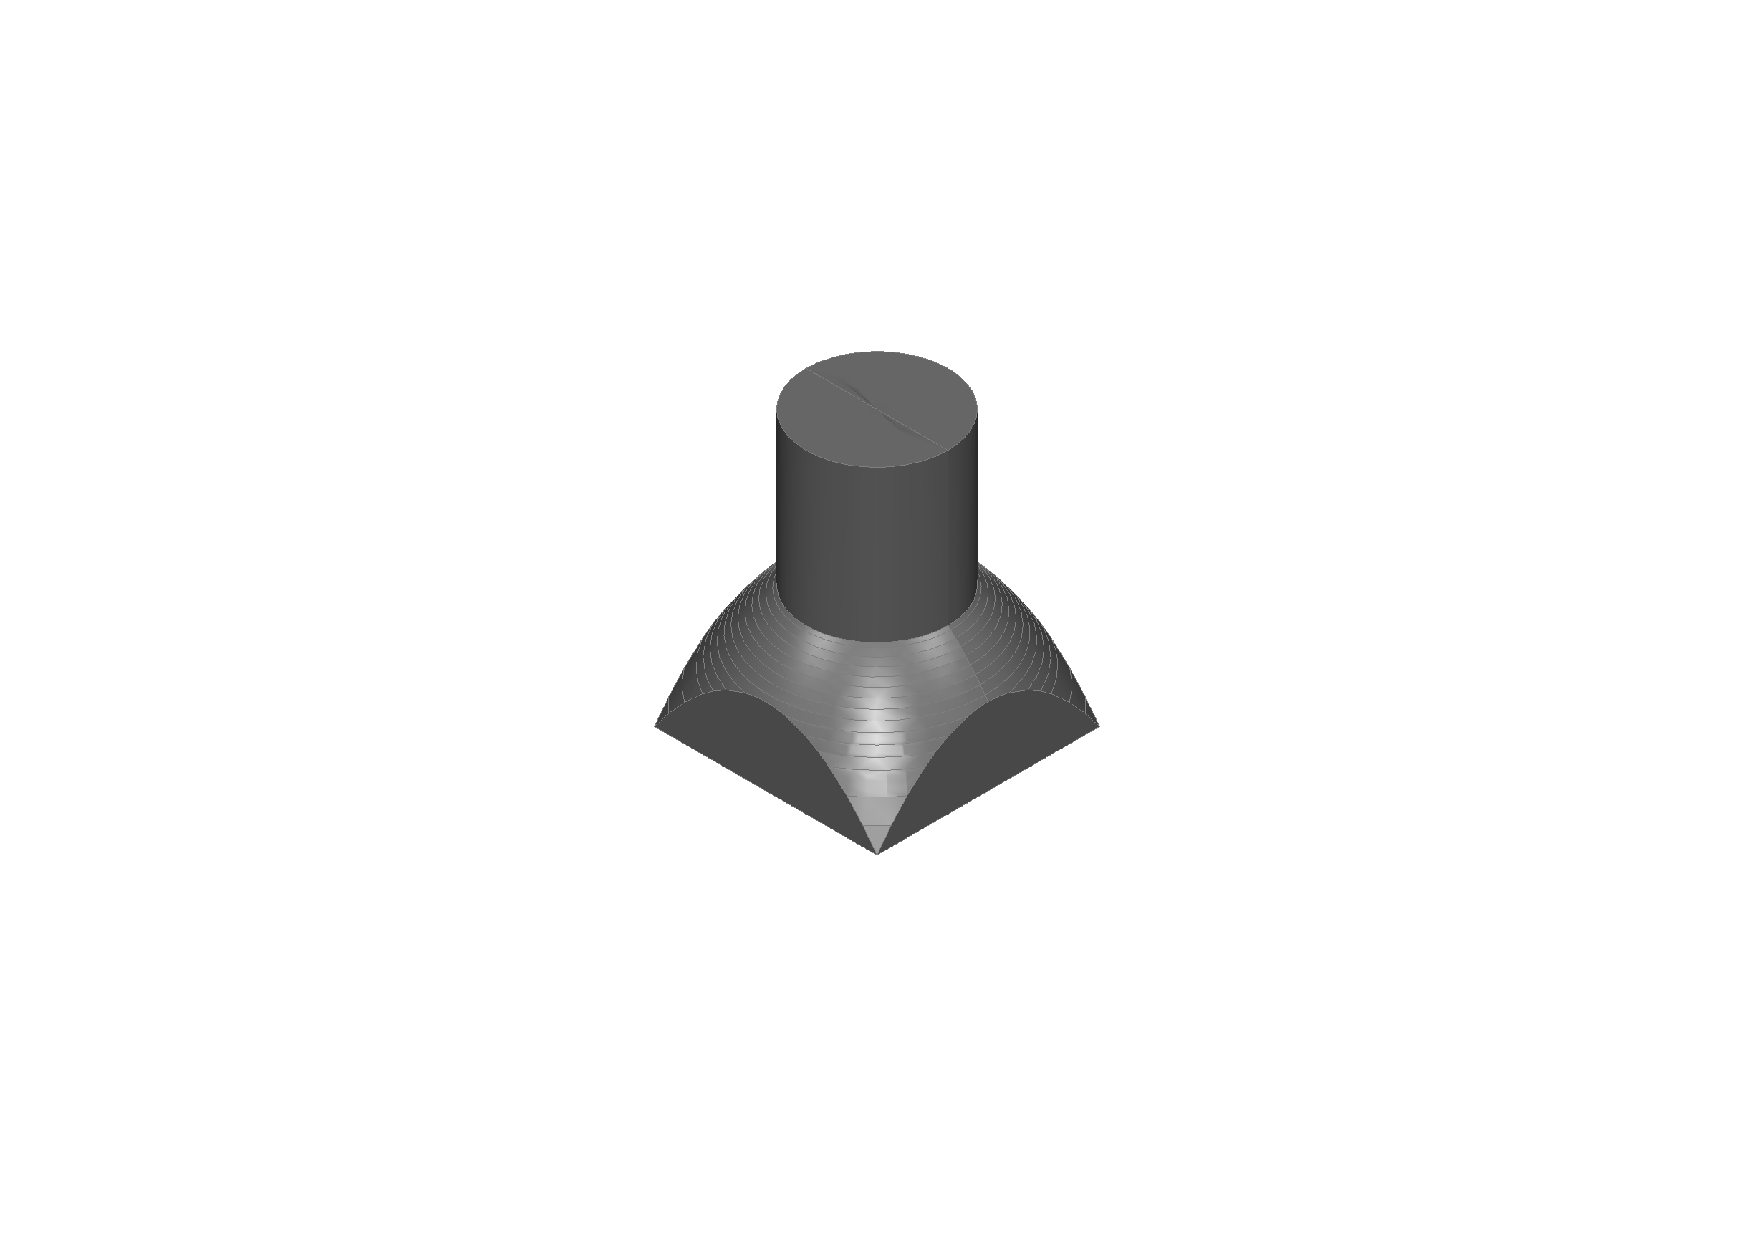
\includegraphics[width=0.45\textwidth]{parts/bar_lg.pdf}
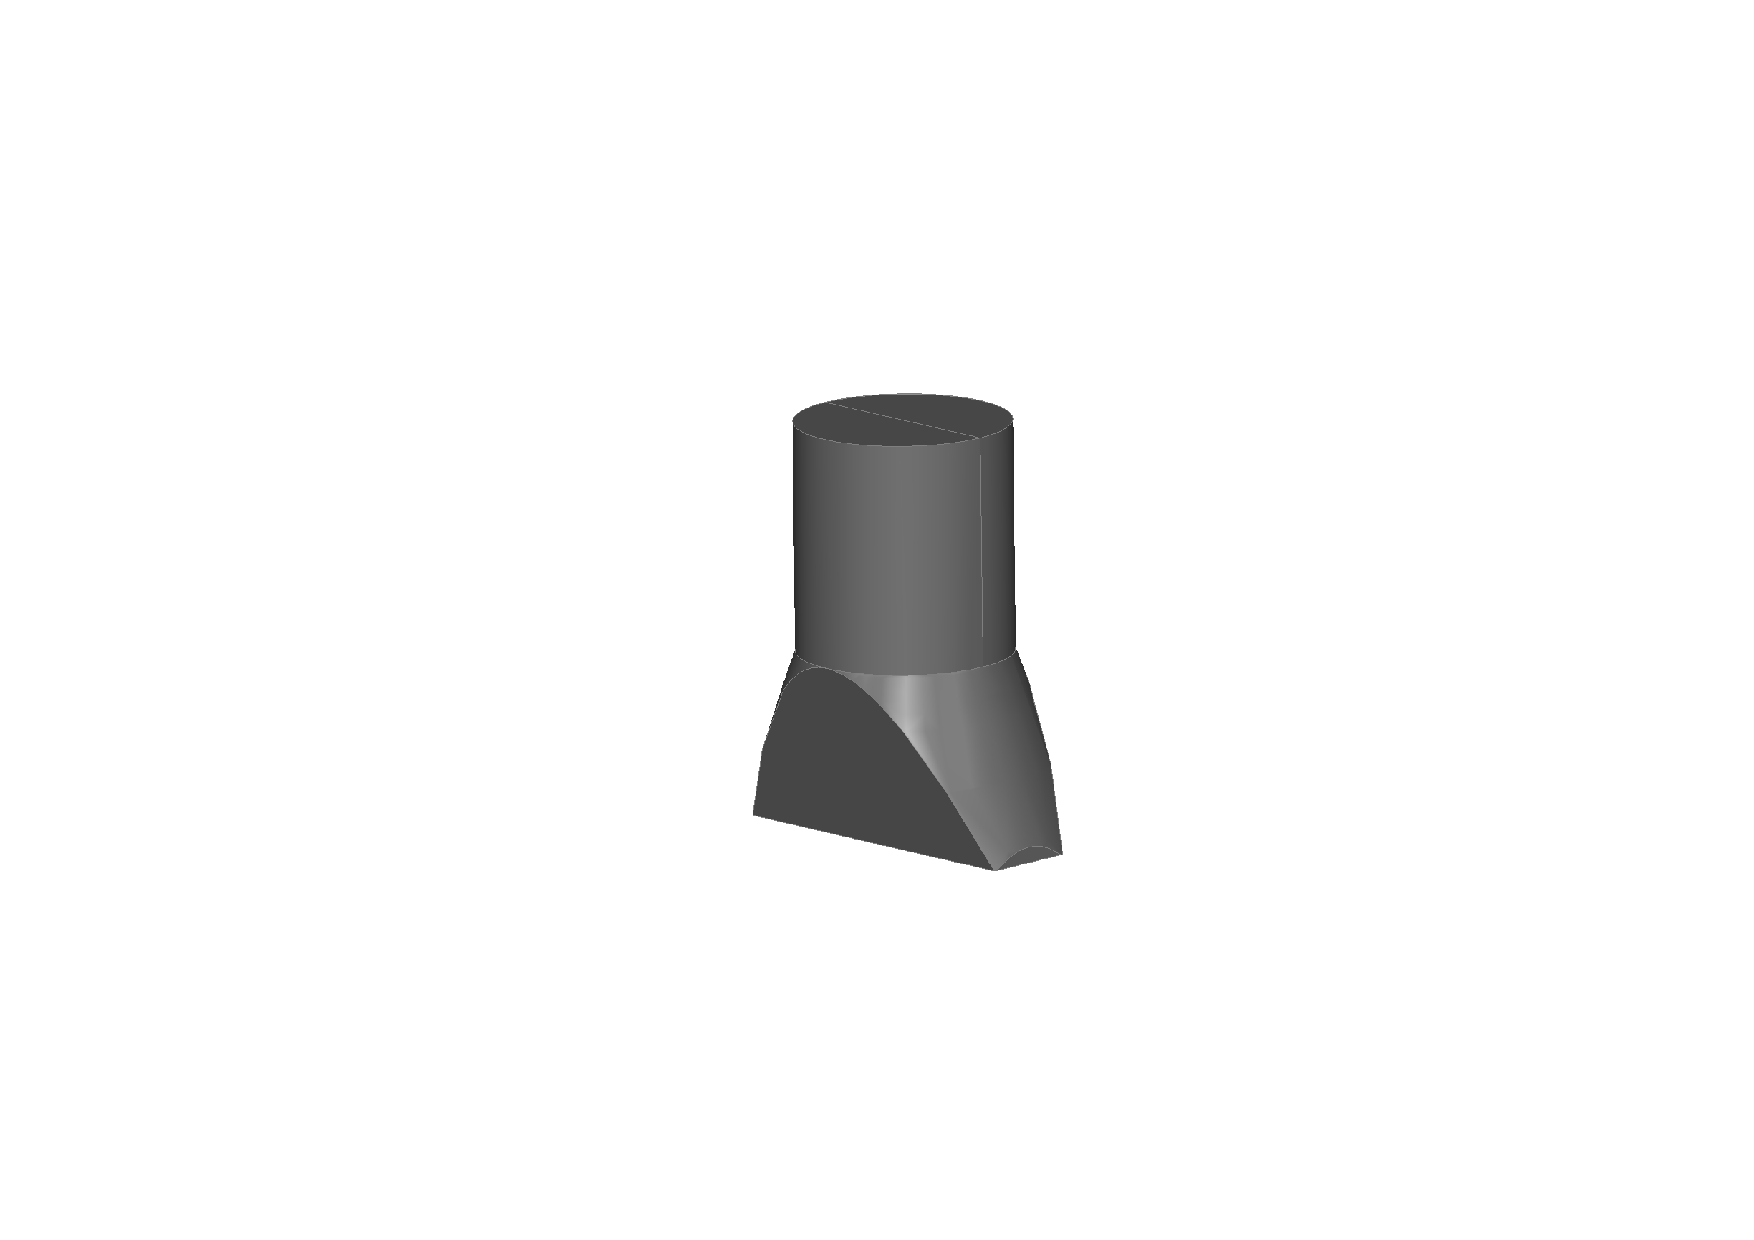
\includegraphics[width=0.45\textwidth]{parts/veto_lg.pdf}
\caption{}
\label{fig:bandlg}
\end{figure}

\item assembly, installation
\item electronics
The total number of channels for BAND including the veto layer is 256. Between BAND and CLAS a $2\,\mathrm{cm}$ lead shield is installed.


In order to operate the PMTs, high voltages (typically in the range of 1500 V) are provided by a multi-channel CAEN SYS4527 mainframe with 11 A1535SN cards (24 channel each).
The signal of each PMT is sent to an splitter. The splitter are the same as the one used by the HPS experiment.
From the splitter one signal is sent to flash-ADCs (250 VXS, 16 channels/board, made and owned by JLab) while the other signal is sent to  discriminators used by HPS (16 channels/board).
The discriminated time signal then goes to a TDC (CAEN VX1190A, 128 channels/board, 100 ps/channel resolution). The read-out system is installed left of BAND in beam direction. 
In total, the system consists of 16 flash-ADCs in one VXS crate, 16 discriminators and a TDC in a VME crate and 16 splitters.  Furthermore, a signal distribution card for the flash-ADCs and trigger interface boards are installed in the crates. A trigger for cosmics for testing and on a pulser for the laser calibration system will be implemented. BAND does not need to be implemented in the main event triggers of CLAS12.


\item laser system
The Laser calibration system consists of a Teem Photonics STV-01E-140 picosecond laser with a wavelength of $355\,\mathrm{nm}$, several splitters, reference photodiode and a fiber distribution system. All of these components are in a sealed, light-tight box. The output of the laser is about $1\,\mu\mathrm{J}$ which will be attenuated and distributed to all fiber outputs which have an output of about $100\,\mathrm{fJ}$. The fibers are connected via a patch panel to each scintillator bar. 

\end{itemize}


% (E.S): I saw we can just quickly summarize the general design considerations in the intro, and leave these about more optimization of detector components and final design chosen
%NOTE: Not sure if this fits here, but the space constraints gave some limitation on the detector design.
%Due to space constraints in HallB, the only possible space closest to the target is on top of the support cart for the silicon vertex tracker of CLAS12.  The detector in context of its surroundings (target, beam line and cart) is shown in Fig. \ref{fig:bandcontext}.

%%%%%%%%%%%%%%%%%%%%%%%%%%%%%%%%%%%%%%%%%%%%%%%%%%%%%%%%%%%%%%%%%%%%%%%%%%%%%%%%%%%%%%%%%%%%%%%%%%%

\section{BAND Performance}

\begin{itemize}
\item bench measurements
Some plots from our most recent measurements in the lab with realistic BAND bars. Laser resolution and maybe a cosmic run.

\item source, cosmic, laser calibrations
\item beam performance
\end{itemize}

% ==================================================================================================
\subsection{Effective Velocity}

The velocity of light traveling through the scintillator bars 
can be determined from the width of the left minus right time spectra for a given bar ($\Delta t$), and the bar length ($L$) as:

\begin{equation}
v_{eff} = \frac{2 \cdot L}{\Delta t}
\end{equation}

% ---------------------------------------------------
\begin{figure}[h!]
\centering
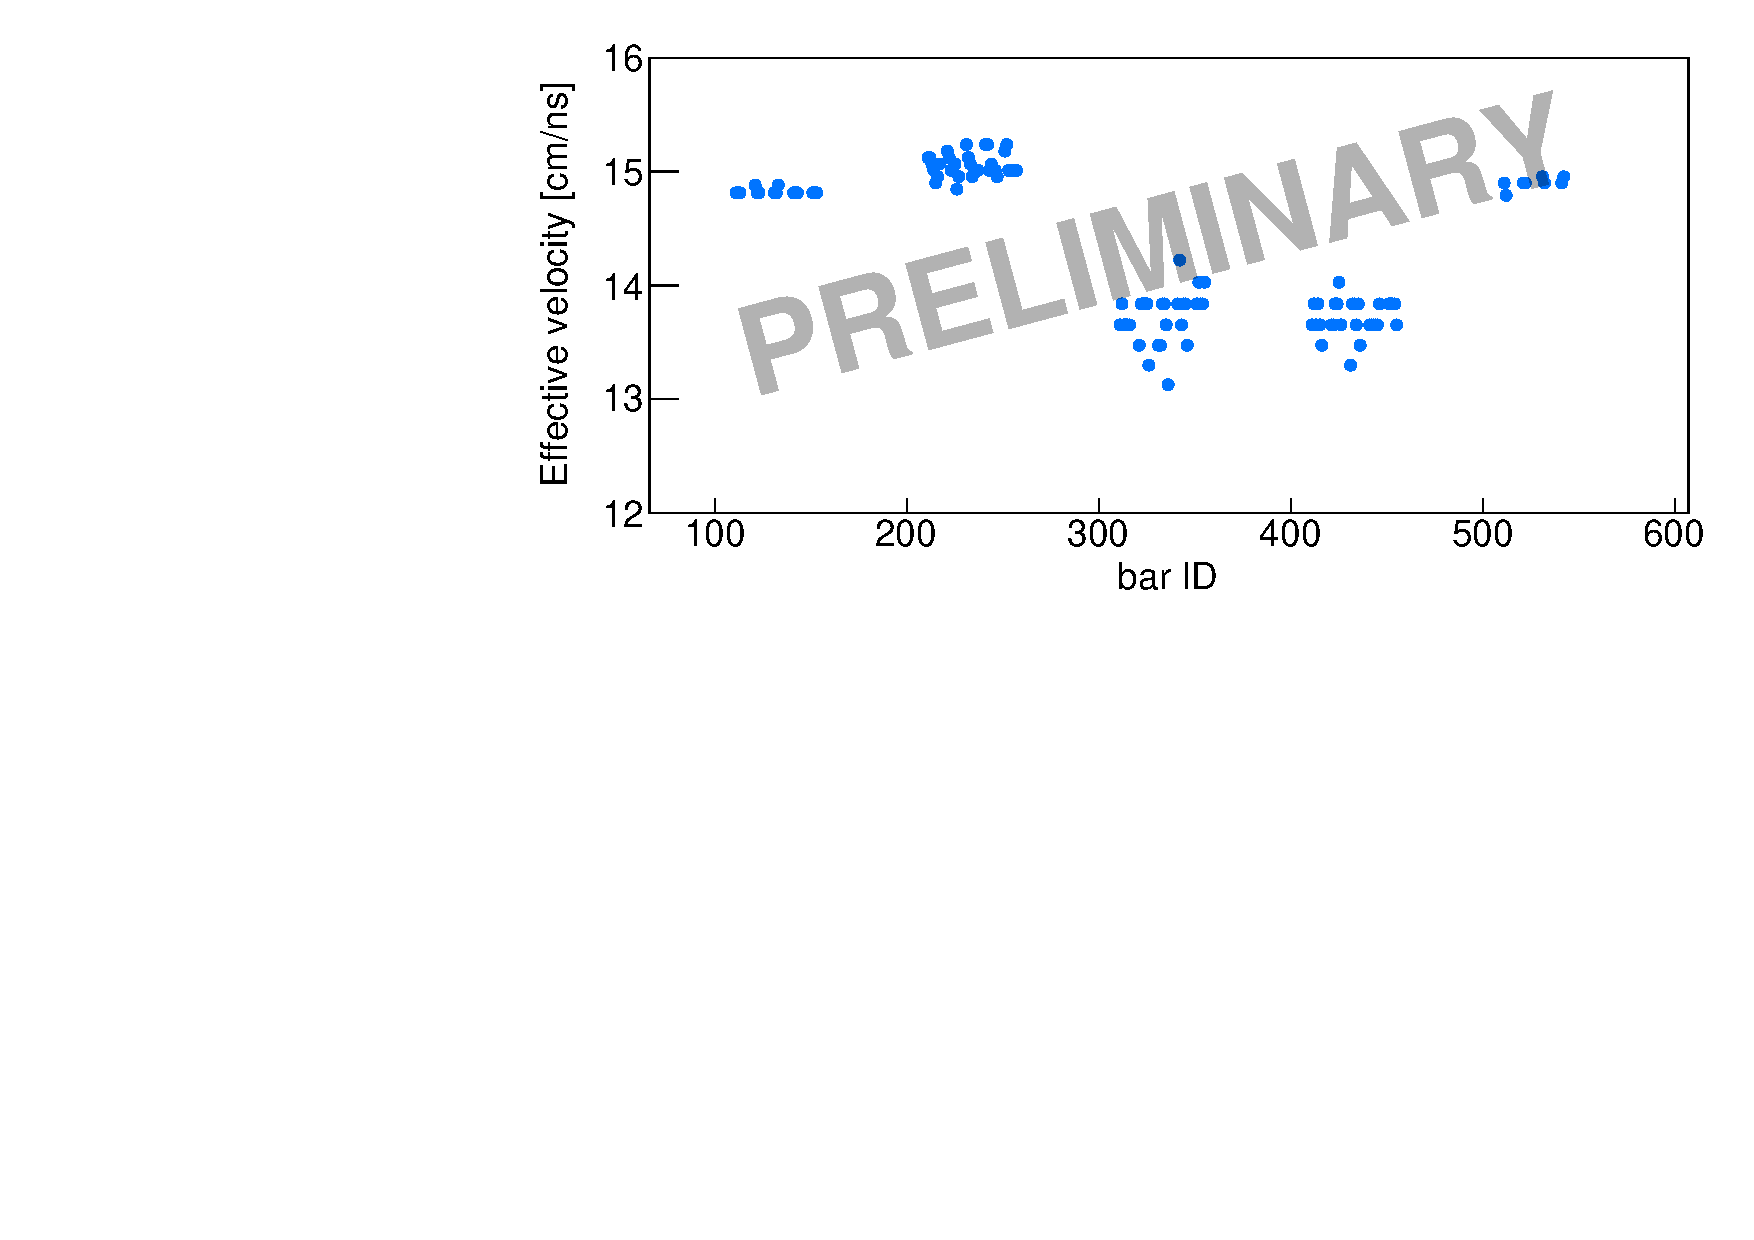
\includegraphics[width=0.8\textwidth]{figures/calibrations/eff_velocity.pdf}
\caption{}
\end{figure}
% ---------------------------------------------------

$\Delta t$ is defined as the the width of the left minus right time spectra at $20\%$ of the maximum of the distribution using cosmic data.

% ==================================================================================================
\subsection{Attenuation Length}

The distance in which the intensity of light traveling through a scintillator drops by $1/e$ is called attenuation length.
It is used to correct the ADC values when determining the deposited energy.
While scintillator manufacturers provide attenuation length values, this value can be significantly different
when a detector is built, and thus it has to me measured.
The attenuation length, hereby denoted by $\mu$, can be related to ADC and timing information recorded by
the left and right PMTs in a given bar as:

\begin{equation}
ln(R) \equiv ln \Big( \frac{\rm{ADC}_L}{\rm{ADC}_R} \Big) = -\frac{v_{eff}}{\mu}(t_L-t_R)
\end{equation}

Consequently, $\mu$ can be determined by fitting a linear function to a plot of $ln ( R )$ vs. $-v_{eff}(t_L-t_R)$
and extracting the inverse of the slope. We carry out this measurement with cosmic data, since cosmic rays
interact with the detector throughout the entire length of the bars (in contrast, for example, with the laser data,
which only produces hits at the center of the bar).

% ---------------------------------------------------
\begin{figure}[h!]
\centering
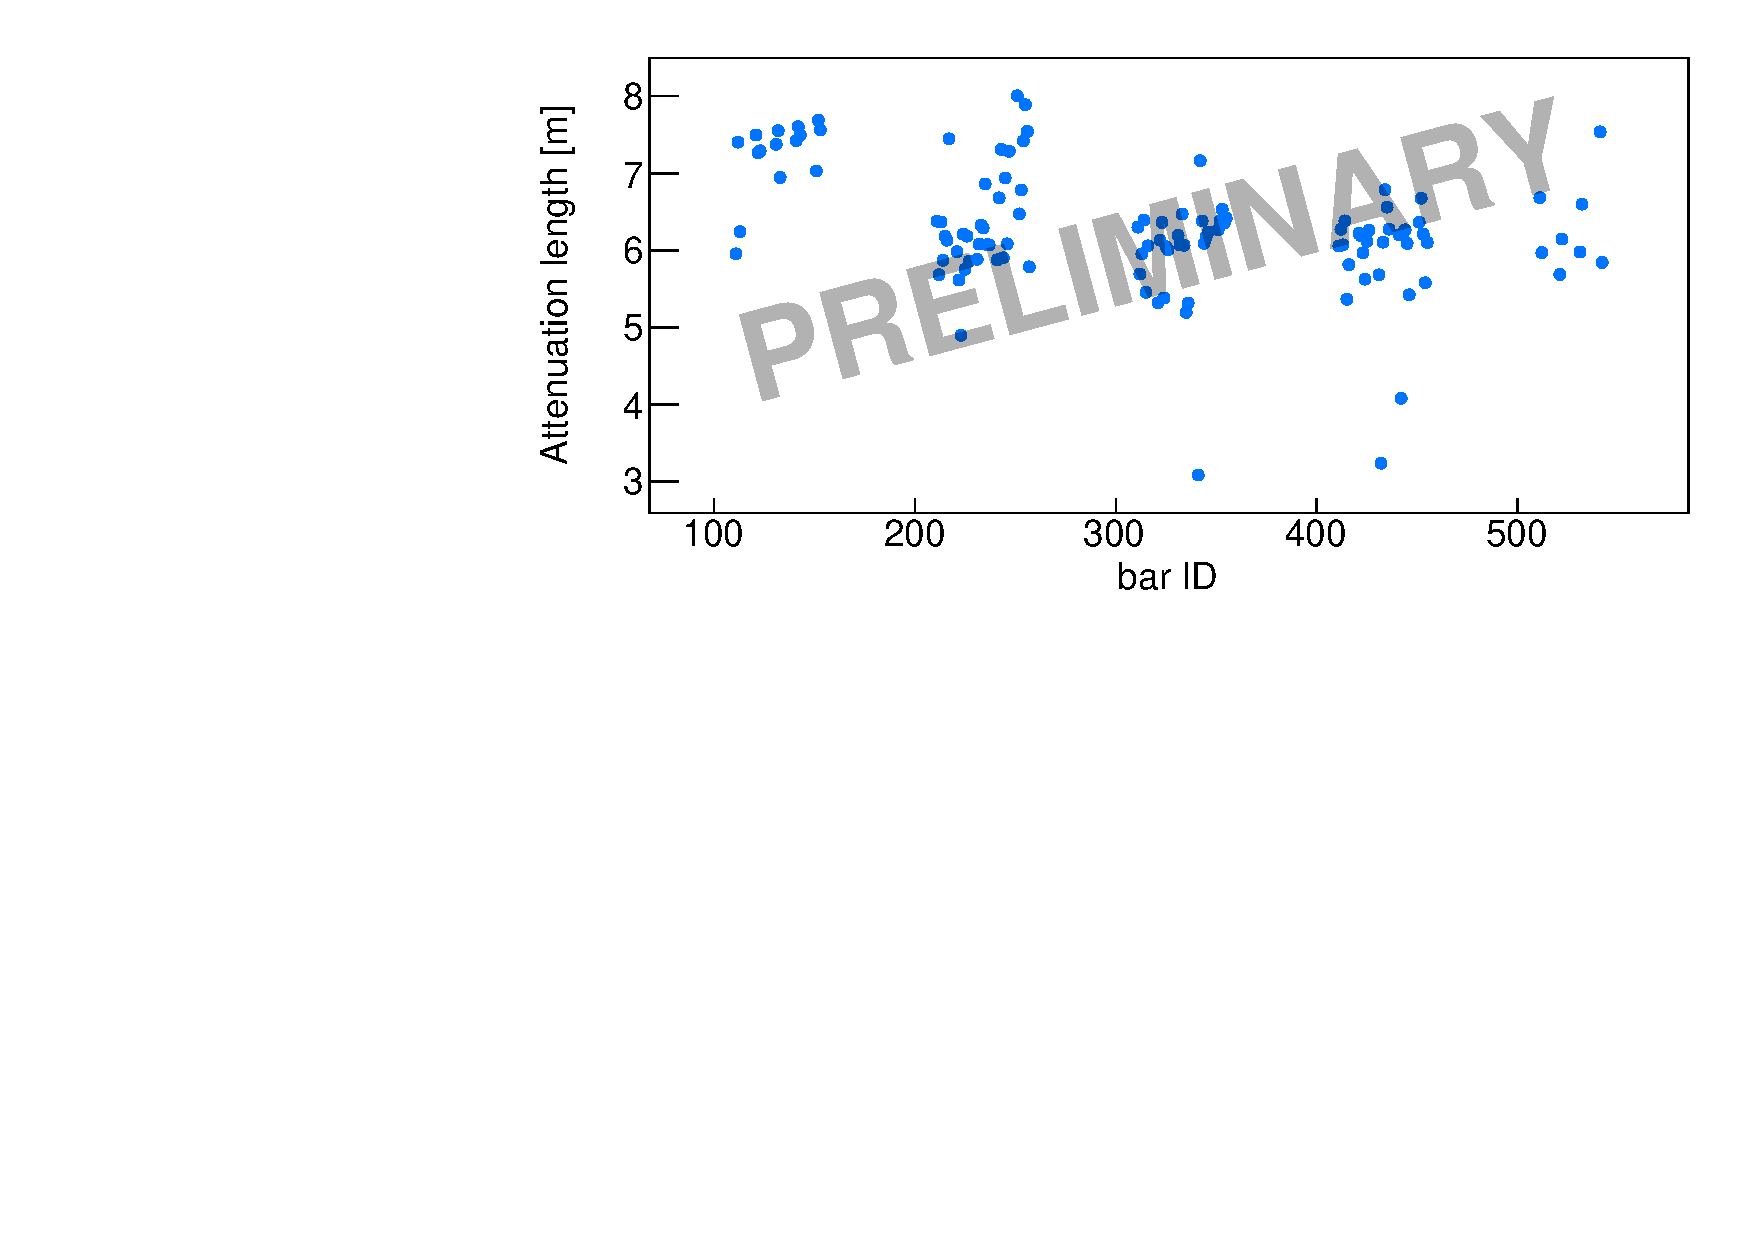
\includegraphics[width=0.8\textwidth]{figures/calibrations/attenuation.pdf}
\caption{}
\end{figure}
% ---------------------------------------------------

% ==================================================================================================
\subsection{Resolution}

% ---------------------------------------------------
\begin{figure}[h!]
\centering
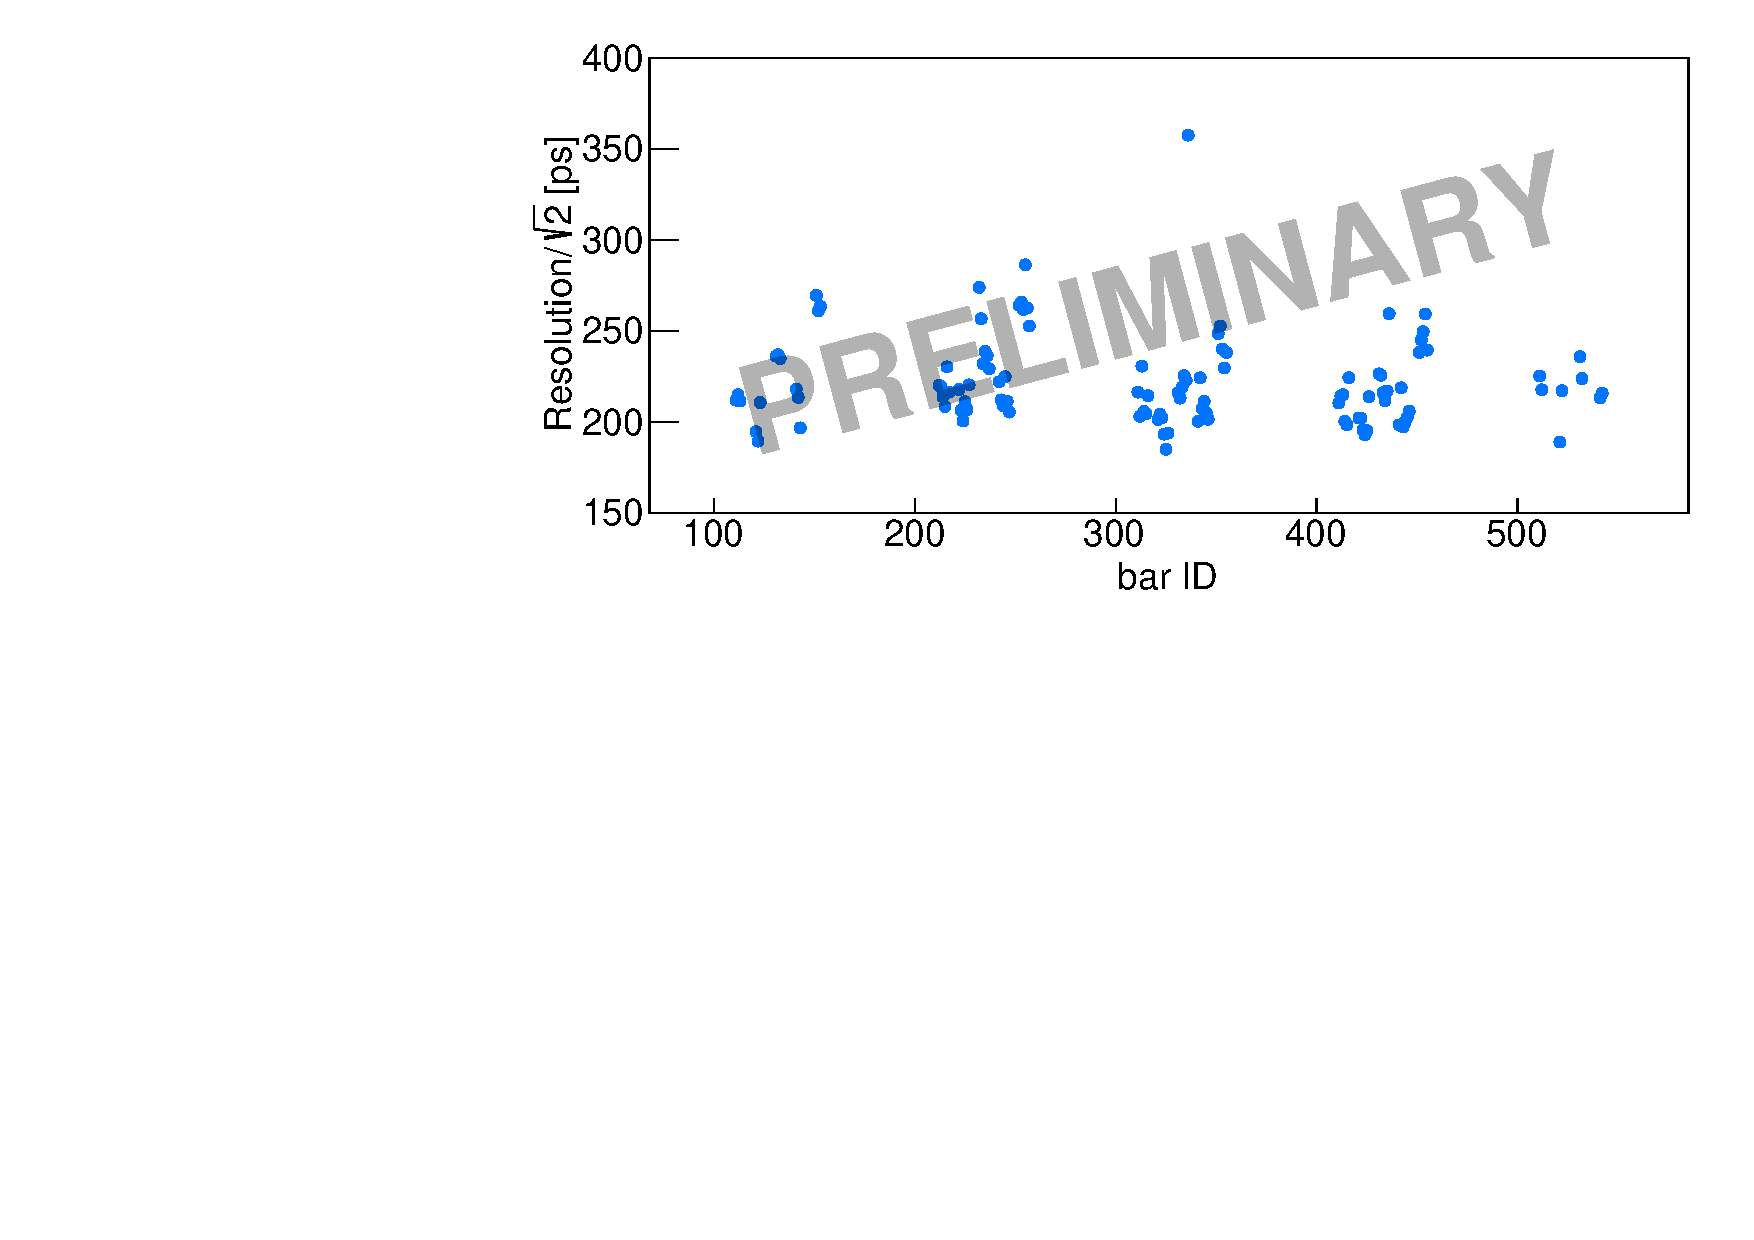
\includegraphics[width=0.8\textwidth]{figures/calibrations/resolutions.pdf}
\caption{}
\end{figure}
% ---------------------------------------------------

%MISSING PICTURE


%%%%%%%%%%%%%%%%%%%%%%%%%%%%%%%%%%%%%%%%%%%%%%%%%%%%%%%%%%%%%%%%%%%%%%%%%%%%%%%%%%%%%%%%%%%%%%%%%%%

\section{Summary}

%%%%%%%%%%%%%%%%%%%%%%%%%%%%%%%%%%%%%%%%%%%%%%%%%%%%%%%%%%%%%%%%%%%%%%%%%%%%%%%%%%%%%%%%%%%%%%%%%%%

\section{Acknowledgements}

%%%%%%%%%%%%%%%%%%%%%%%%%%%%%%%%%%%%%%%%%%%%%%%%%%%%%%%%%%%%%%%%%%%%%%%%%%%%%%%%%%%%%%%%%%%%%%%%%%%

\section*{References}
\bibliography{mybibfile}


\end{document}